\newpage
\section{Coupling to numerical models} \label{s:coupling}

CPlantBox is a bottom up model where no water movement or solute transport is calculated per default. The idea is to make it easy to link the root growth model to any numerical models or solvers. This is achieved by member functions that make it easy to (a) obtain a numerical grid from the root system, and (b) to offer utility functions to map root segments to an underlying soil grid. 

In this section we consider a static root system. The additional steps that are needed for a developing root system (i.e. with a changing root geometry) are explained in the next section. 

\subsection{Mapping between root segments and an underlying soil} \label{ss:mapping}

The classes MappedSegments and MappedRootSystem, defined in MappedOrganism.h, manage the coupling between the root system and external models or solvers. 

The RootSystem class stores the nodes of each root in an object of class Root. This is convenient for simulating the root development, but not suitable for coupling to numerical models. Commonly, numerical models need the nodes as sequential list (obtained by RootSystem::getNodes) and the information on how they are connected (e.g. RootSystem::getSegments). Additionally, some information on the segments like radius or root type is needed. Furthermore, when coupling to a soil model, we need information in which soil cell the segment is located, and vice versa, which segments are located within a specific soil cell. 

The class MappedSegments helps to manage all that, and offers the data structure for sequential nodes, connections between two nodes as segments, and the most commonly needed data such as creation time of the node, and radius or type per segment. Most important, it contains two hash maps seg2cell and cell2seg, linking segments to cells, and cells to list of segments.

MappedRootSystem is derived from MappedSegments and RootSystem, i.e. it can be used in the exact same way as the RootSystem class, but keeps track of the lists, and (optionally) the mapping between soil grid and root system.

To demonstrate basic functionality we will map a root system to a soil rectangular soil grid. 

\lstinputlisting[firstline=1, language=Python, caption=Example 6a]{../../examples/python/example6a_mapping.py}

\begin{itemize}

\item[8-12] Creation of a small root system. Instead of the class RootSystem, MappedRootSystem is used (L8). MappedRootSystem is a specialisation of the 'normal' RootSystem class and can be used in the exactly same way. 

\item[16-19] We choose a small soil domain, where some roots are not inside. Calling MappedRootSystem::setRectangularGrid first cuts segments at the cell faces, and then maps the resulting segments to a soil index (creates the maps MappedRootSystem::seg2cell, and MappedRootSystem::cell2seg). The value True indicates that cutting is performed, False just maps the segment mid points without cutting. 

\item[22-28] Next we create an array $x$ containing the soil indices for each segment, that will be later used for vizualisation. We use the hash map (a Python dictionary) MappedRootSystem::seg2cell to obtain the linear index of the cell, where the segment's mid point is located.

\item[31-37] To demonstrate how to retrieve all segments that lie within a given cell, we output the segments at the cell located around the position [0,0,-7]. In L31 we retrieve the cell index for that position. L34 and L35 print out the segment indices. Note that the map will have no entry for a given cell, if no segments are located in the cell. 

\item[43-48] To visualize the soil cell indices, we first create a SegmentAnalyser class. The class MappedRootSystem is derived from a RootSystem and MappedSegments. If we create a SegmentAnalyser class directly from $rs$ (L40) MappedRootSystem will be considered as RootSystem, and the resulting class will contain the original segments before cutting at the cell boundaries. The function MappedRootSystem::mappedSegments (L41) will return a reference to $rs$ but with the type MappedSegments. In this way the SegmentAnalyser class will be created including the cut segments. Next, in L42 we add the indices as data to the SegmentAnalyser class. L43, L44 produces the VTK plot, but rendering is started at a later point, since we also want to visualize the underlying soil grid.

\item[51-53]  L47 creates the mesh for vizualisation, L48 creates the VTK plot, and L49 starts the rendering window, rendering both, root system and underlying soil. Press 'y', 'x', and 'z' to obtain axis aligned views of the root system and soil grid.

\end{itemize}

More, generally, when coupling to an external solver like DuMux \citep{koch2020dumux}, we need to set the soil$\_$index function, that returns the cell index for a certain position. Additionally, periodic soil domains are already implemented. Both coupling to DuMux and periodicity will be demonstrated in Section \ref{sec:dumux_coupling}.

Coupling to an unstructured grid is as simple as to a structured one. But automatic cutting of segments at the cell faces is currently not implemented. That means that axial resolution should be small in order to keep the introduced error small.



\subsection{Water movement within the roots} \label{ssec:xylem}

Since water movement within the roots is often needed, it is implemented directly in CPlantBox (in the class XylemFlux) following \cite{meunier2017hybrid}. However, usage is optional, and any other transport code can be used (e.g. if solutes are considered). XylemFlux sets up the linear system, and the sparse linear system is then solved in Python using scipy (using the class XylemFluxPython defined in xylem$\_$flux.py).

The following example is based on benchmark M3.1 \citep{schnepf2019call} with constant conductivities, but not with a given root system, but a simulated one.

\lstinputlisting[firstline=1, language=Python, caption=Example 6b]{../../examples/python/example6b_xylemflux.py}
\begin{itemize}

\item[11-15] All parameters that will be used later on.

\item[18-23] The root system (similar to last section). 

\item[26-31] The MappedRootSystem is wrapped with the XylemFluxPython class, which extends the XylemFlux class, which computes the xylem matric flux potential. L27, L28 sets the radial and axial conductivity. L29 retrieves the root system nodes for later visualisation. The pressure surrounding the the root system is either defined as pressure surrounding each root segment, or as soil cells, in which the root segments are located. L30, L31 sets a soil containing of one single cell with index 0. 

\item[34-36] XylemFluxPython defines solvers like solve$\_$dirichlet for Dirichlet boundary condition (predefined collar matric potential), solve$\_$neumann for Neumann boundary condition (predefined collar flux), and solve which switches between Dirichlet and Neumann at some critical pressure (the plant wilting point).
The arguments of solve$\_$dirichlet are the simulation time (to calculate age dependent conductivities), the root collar pressure head, the pressure around the root collar, the soil matric potential around the root segments or per soil cell, and a boolean value that decides if the potentials are given per soil cell (True) or per segments (False). The return value $rx$ contains the xylem matric potentials per segment. L35 calculates the fluxes into the soil (negative values mean into the root). The bool argument determines if we approximate the flux, or use the exact solution by \cite{meunier2017hybrid}.
L36 determines the root collar flux.

\item[39-43] Plots the results.

\item[46-49] Creates the VTK plot, adding the soil matric potentials and fluxes. L49 picks either $rx$ or $fluxes$ for vizualisation, see Figure \ref{fig:xylemfluxa} and \ref{fig:xylemfluxb}.

\end{itemize}

It is possible to set conductivties per root type (see XylemFlux::setKr, and setKx), and root age dependent conductivities per root type using linear lookup tables (see XylemFlux::setKrTables, and setKxTables).

\begin{figure}
\begin{subfigure}[c]{0.5\textwidth}
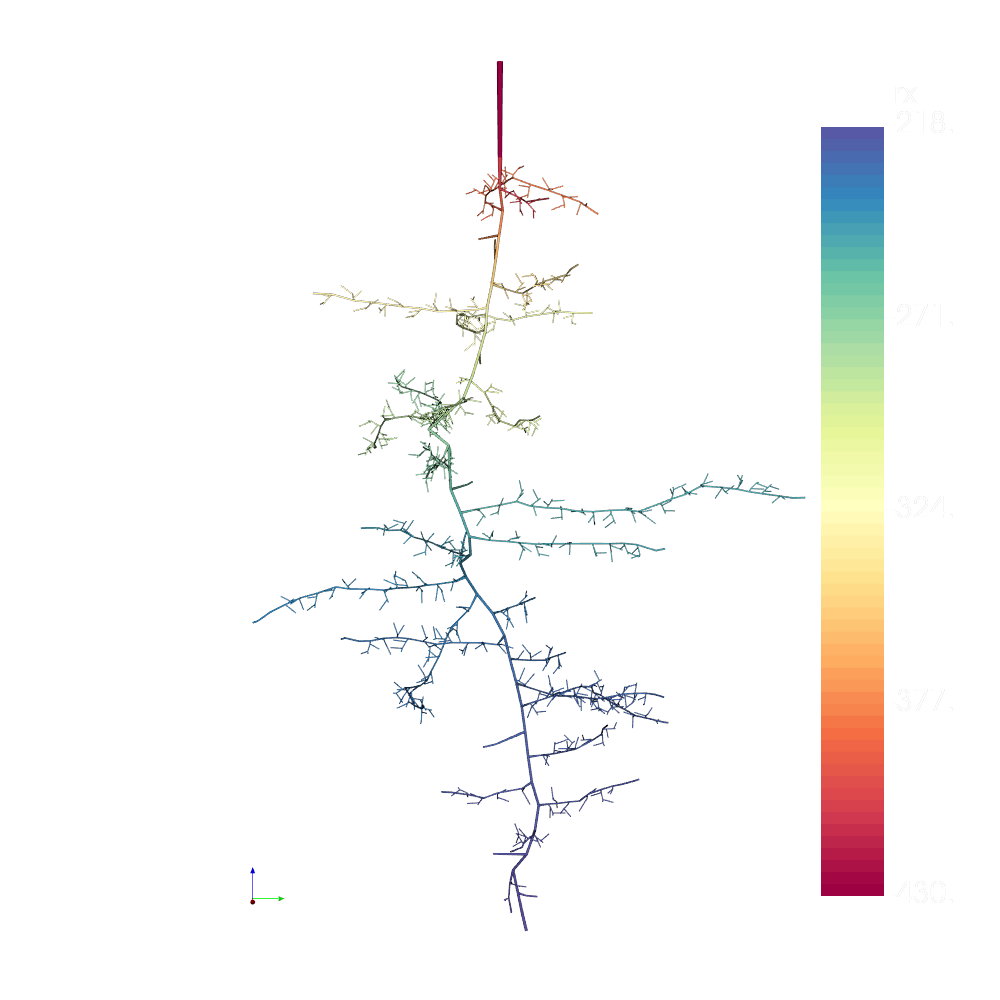
\includegraphics[width=0.99\textwidth]{example6b.png}
\subcaption{Anagallis} \label{fig:xylemfluxa}
\end{subfigure}
\begin{subfigure}[c]{0.5\textwidth}
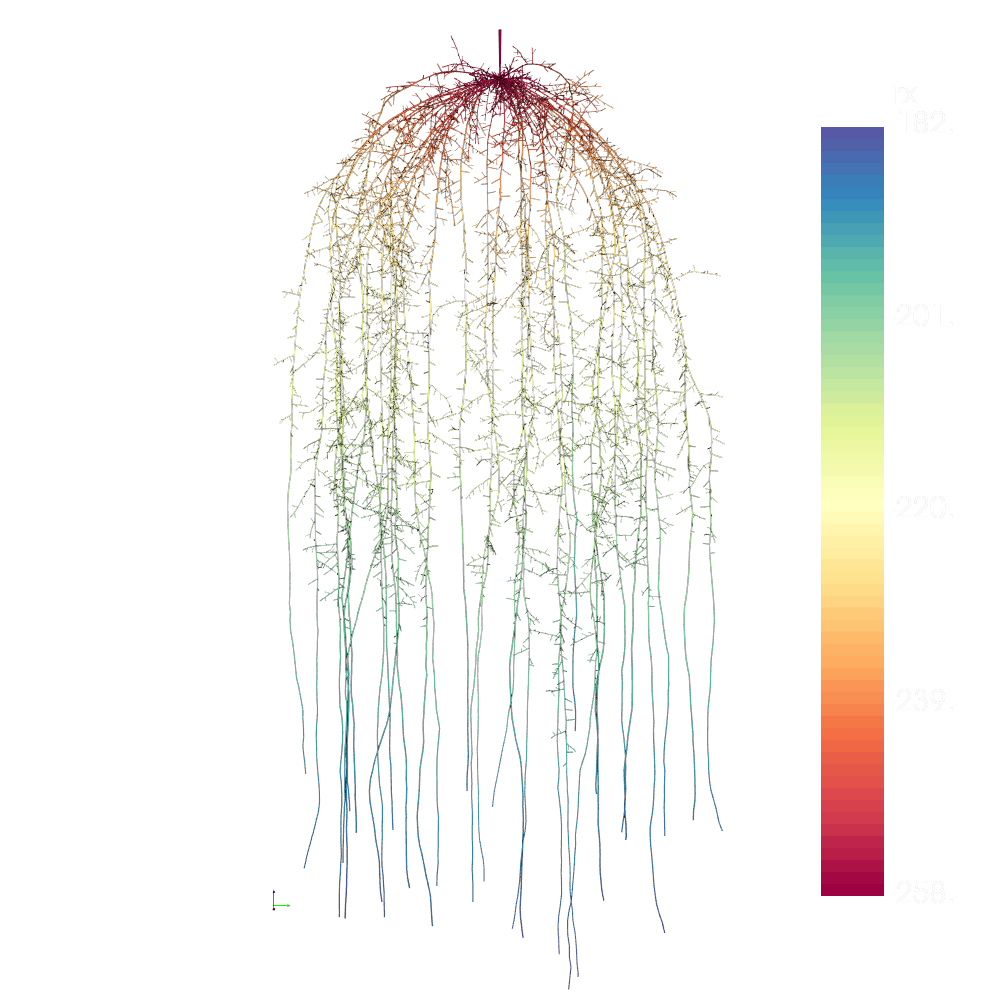
\includegraphics[width=0.99\textwidth]{example6b_2.png}
\subcaption{Maize} \label{fig:xylemfluxb}
\end{subfigure}
\caption{Calculated xylem matric potential (cm)} 
\end{figure}

\subsection{Stomatal modul} \label{ssec:stomatal}

The following example presents the stomatal modul (see file example6e$\_$xylemflux$\_$variable$\_$gs.py). The actual evapotranspiration (ETa) of the plant is determined according to environmental parameters, root and leaf surface, and maximal stomatal conductance (gmax). 
\lstinputlisting[firstline=1, language=Python, caption=Example 6e]{../../examples/python/example6e_xylemflux_variable_gs.py}
\begin{itemize}

\item[11-19] Part of the parameters that will be used later on.

\item[18-23] The root system (similar to last section). 

\item[21-25] Creation of the plant object, definition of the grid and simulation of the plant growth.

\item[38-42] Set the parameters for the calculation of the actual leaves radial conductivity (gs) and ETa using the equations of [TOADD].

\item[44-48] Get the plant nodes and tips to set the Neumann boundary conditions (i.e. 0 axial flux is set at the plant nod tips (i.e: water only enters/leaves the plant by radial flux)

\item[51] Solve the water flux using the Neumann boundary conditions. The program then loops on the calculation of ETa, xylem potential, and gs until convergence or after having done 1000 loops. p$\_$linit and gmax are respectively the initial leaf xylem potential and initial leaf radial conductivity used in the loop.

\item[52] Calculation of the radial fluxes of each plant segment.

\item[53] Gives an overview of the water fluxes in the plant. If show$\_$matrices = True, the matrices with the axial and radial water fluxes for each plant segment is shown.

\item[62-72] Plots the results (see Figure \ref{fig:stomata} and \ref{fig:stomatb}).

\item[75-78] Creates the VTP file, which can then be opened in Paraview.

\end{itemize}

\begin{figure}
\begin{subfigure}[c]{0.5\textwidth}
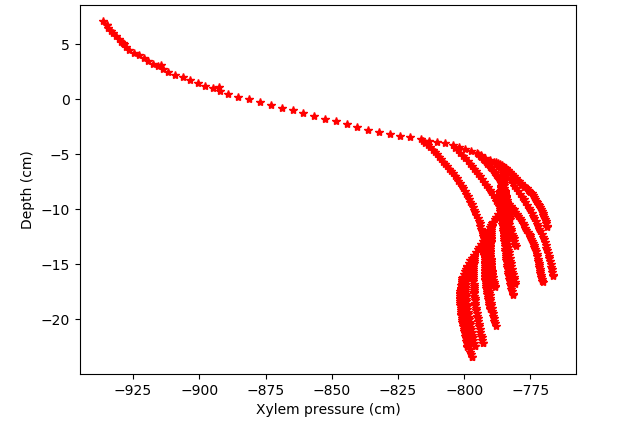
\includegraphics[width=0.99\textwidth]{example6e.png}
\subcaption{Calculated xylem matric potential (cm)} \label{fig:stomata}
\end{subfigure}
\begin{subfigure}[c]{0.5\textwidth}
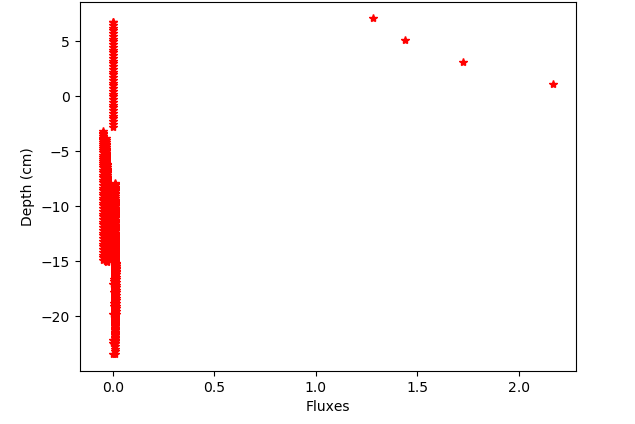
\includegraphics[width=0.99\textwidth]{example6e_2.png}
\subcaption{Radial water fluxes} \label{fig:stomatb}
\end{subfigure}
\caption{xylem potential and radial water fluxes per segment} 
\end{figure}

\subsection{Coupling a static root system to DuMux} \label{sec:dumux_coupling}

Putting the sections \ref{ss:mapping} and \ref{ssec:xylem} together, we can easily set up an example, using the classic sink term in the soil model, similar as in \citep{leitner2014impact} based on \citep{doussan1998modelling}. For solving the Richards equation we use DuMux \citep{koch2020dumux}.

The next example mimics benchmark C12 \citep{schnepf2019call}, but with a static simulated root system. The example must be run out of dumux-rosi (located in dumux-rosi/rosi$\_$benchmarking/python$\_$solver/coupled), otherwise the DuMux Python coupling is not available. 

\lstinputlisting[firstline=1, language=Python, caption=Example 6c]{../../examples/python/example6c_coupling.py}

\begin{itemize}

\item[3,4] Add paths for DuMux Python coupling (L3) and Python solvers (L4).

\item[5,6] The direct C++ part of the DuMux binding, and the Python wrapper class. 

\item[17,18]  Defines a sinusoidal function for the collar boundary condition.

\item[21-37] All parameters that are needed for this simulation. L25 decides if periodic boundary conditions are used, or not. L35 states the simulation time, L36 the initial root system age. L37 defines if age dependent root conductivities are used. The rooot conductivities are hard coded in the file root\_conductivities.py, that is imported in L8. Age dependent conductities can be used to mimic root growth in a predefined way, i.e. the root system is already fully grown, but the radial conductivities are turned on during the simulation. 

\item[41-49] Sets up the soil solver (DuMux Python binding from dumux-rosi). 

\item[52-62] Sets up the Xylem model as in Subsection \ref{ssec:xylem}. If the root system is not periodic, a confining geometry is set L54-L58. L62 passes the axial and radial conductivities to the XylemFluxPython object (the function is defined in root\_conductivities.py).

\item[65-70] Coupling between the soil soil and root part is performed by setting the picking function that assigns a cell index to each spatial position L65, and L66. In L67 root segments are cut to the rectangular grid, and in L70 the cell index of the root collar is determined. 

\item[73-77] Initializes the simulation, initially the soil values are the same as the initial conditions (L75).

\item[79-94] First, we calculate the xylem matric potential $rx$ for a given soil matric potential $sx$ (L81) and save the actual collar flux for later analysis (L83). Next, we calculate teh sink (L85) and apply it to the soil model (L86). The soil model is simulated (L87) and the resulting matric potential $sx$ is updated (L88). The simulation takes some time (around 15 minutes), and L90-93 print debugging information and a progress bar. L94 increases the current simulation time. This is needed if age dependent conductivities are used. 

\item[99-111] L99 creates Figure \ref{fig:example6c} and, L102-111 plots uptake and cumulative uptake over time, see Figure \ref{fig:uptake}.

\end{itemize}

\begin{figure}
\begin{subfigure}[c]{0.5\textwidth}
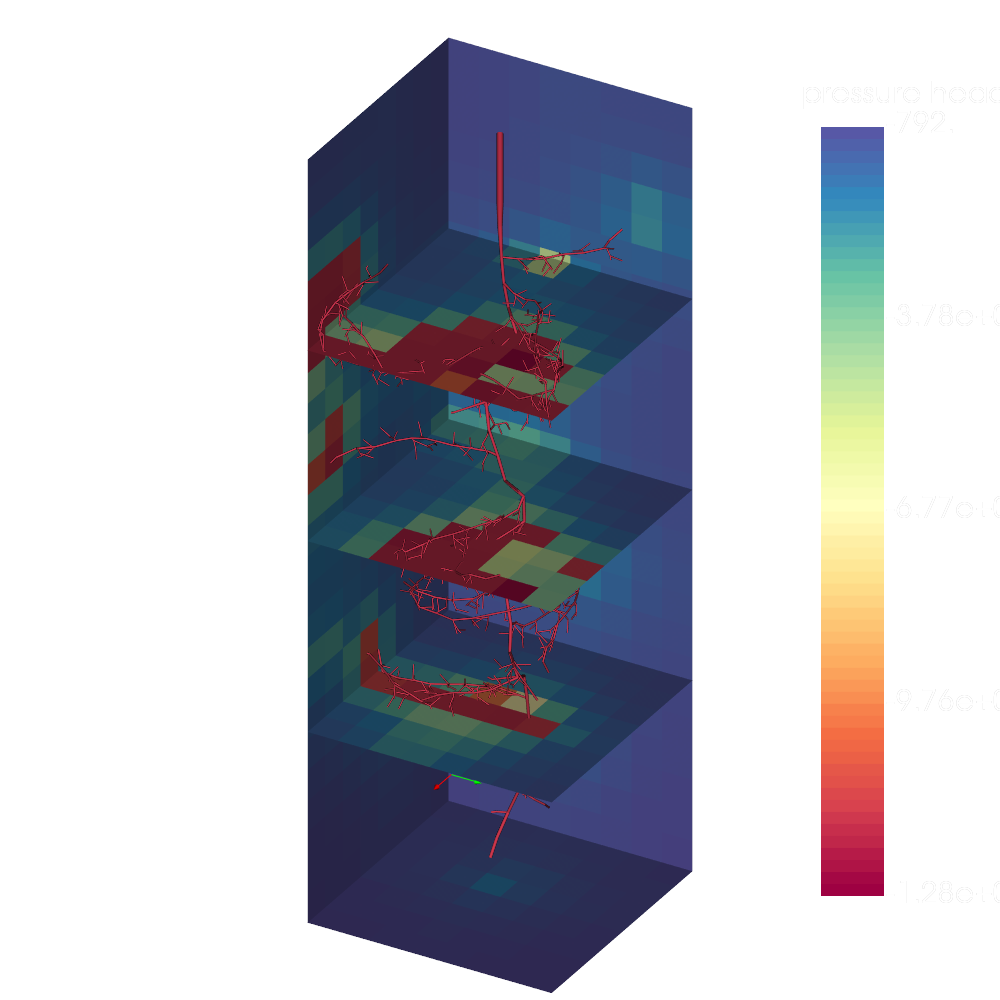
\includegraphics[width=0.99\textwidth]{example6c.png}
\subcaption{Confined} \label{fig:example6c}
\end{subfigure}
\begin{subfigure}[c]{0.5\textwidth}
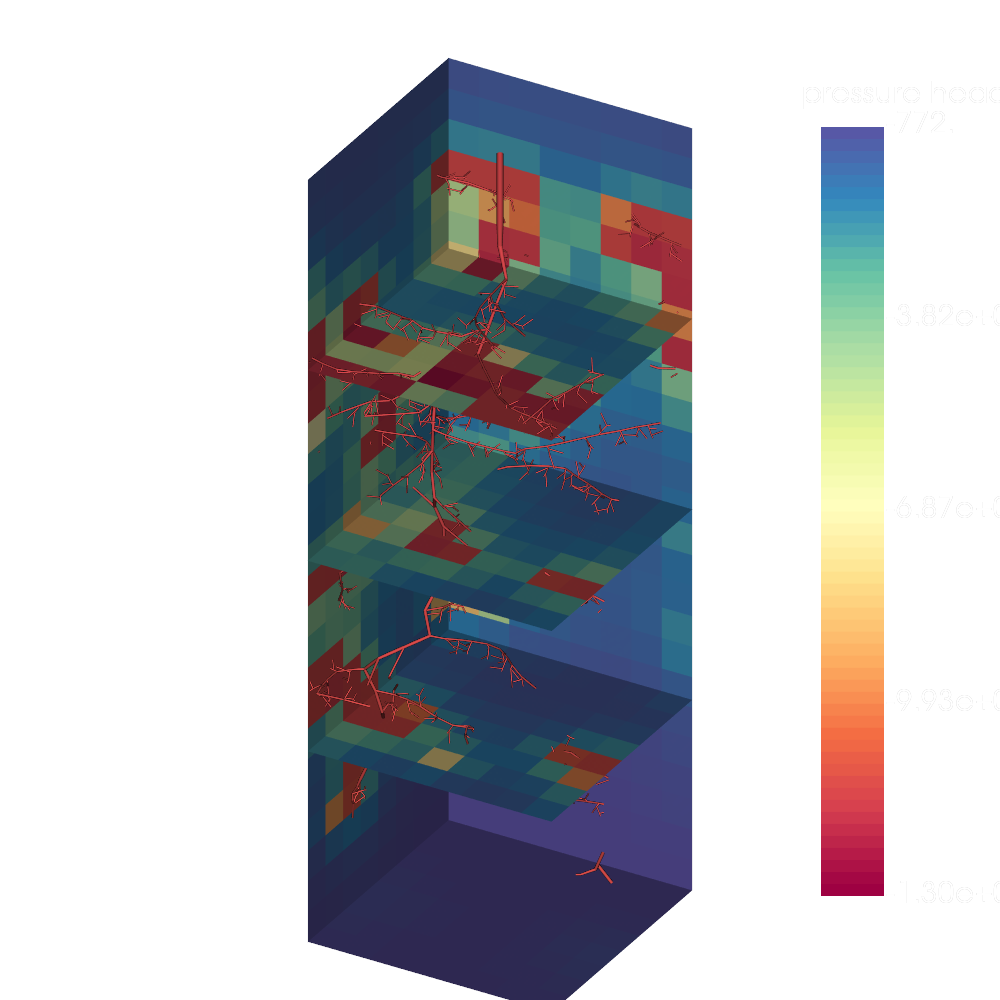
\includegraphics[width=0.99\textwidth]{example6c_periodic.png}
\subcaption{Periodic boundary condtions} \label{fig:example6c_peridodic}
\end{subfigure}
\caption{Water depletion due to root uptake after one week. } \label{fig:example6c}
\end{figure}

With above code we can compare total root system water uptake in a container, with the uptake if periodic boundary conditions are used. While the first scenario reflects the situation in a plant pot, periodic boundary conditions reflect the situation when the plant grows in the field, where the planting distance is approximately the domain size. Figure \ref{fig:uptake} shows both situations, showing that the boundary conditions will strongly affect total water uptake, because roots are less evenly distributed in the pot scenario and water redistribution is impeded by the pot boundaries.

\begin{figure}
\begin{subfigure}[c]{1\textwidth} 
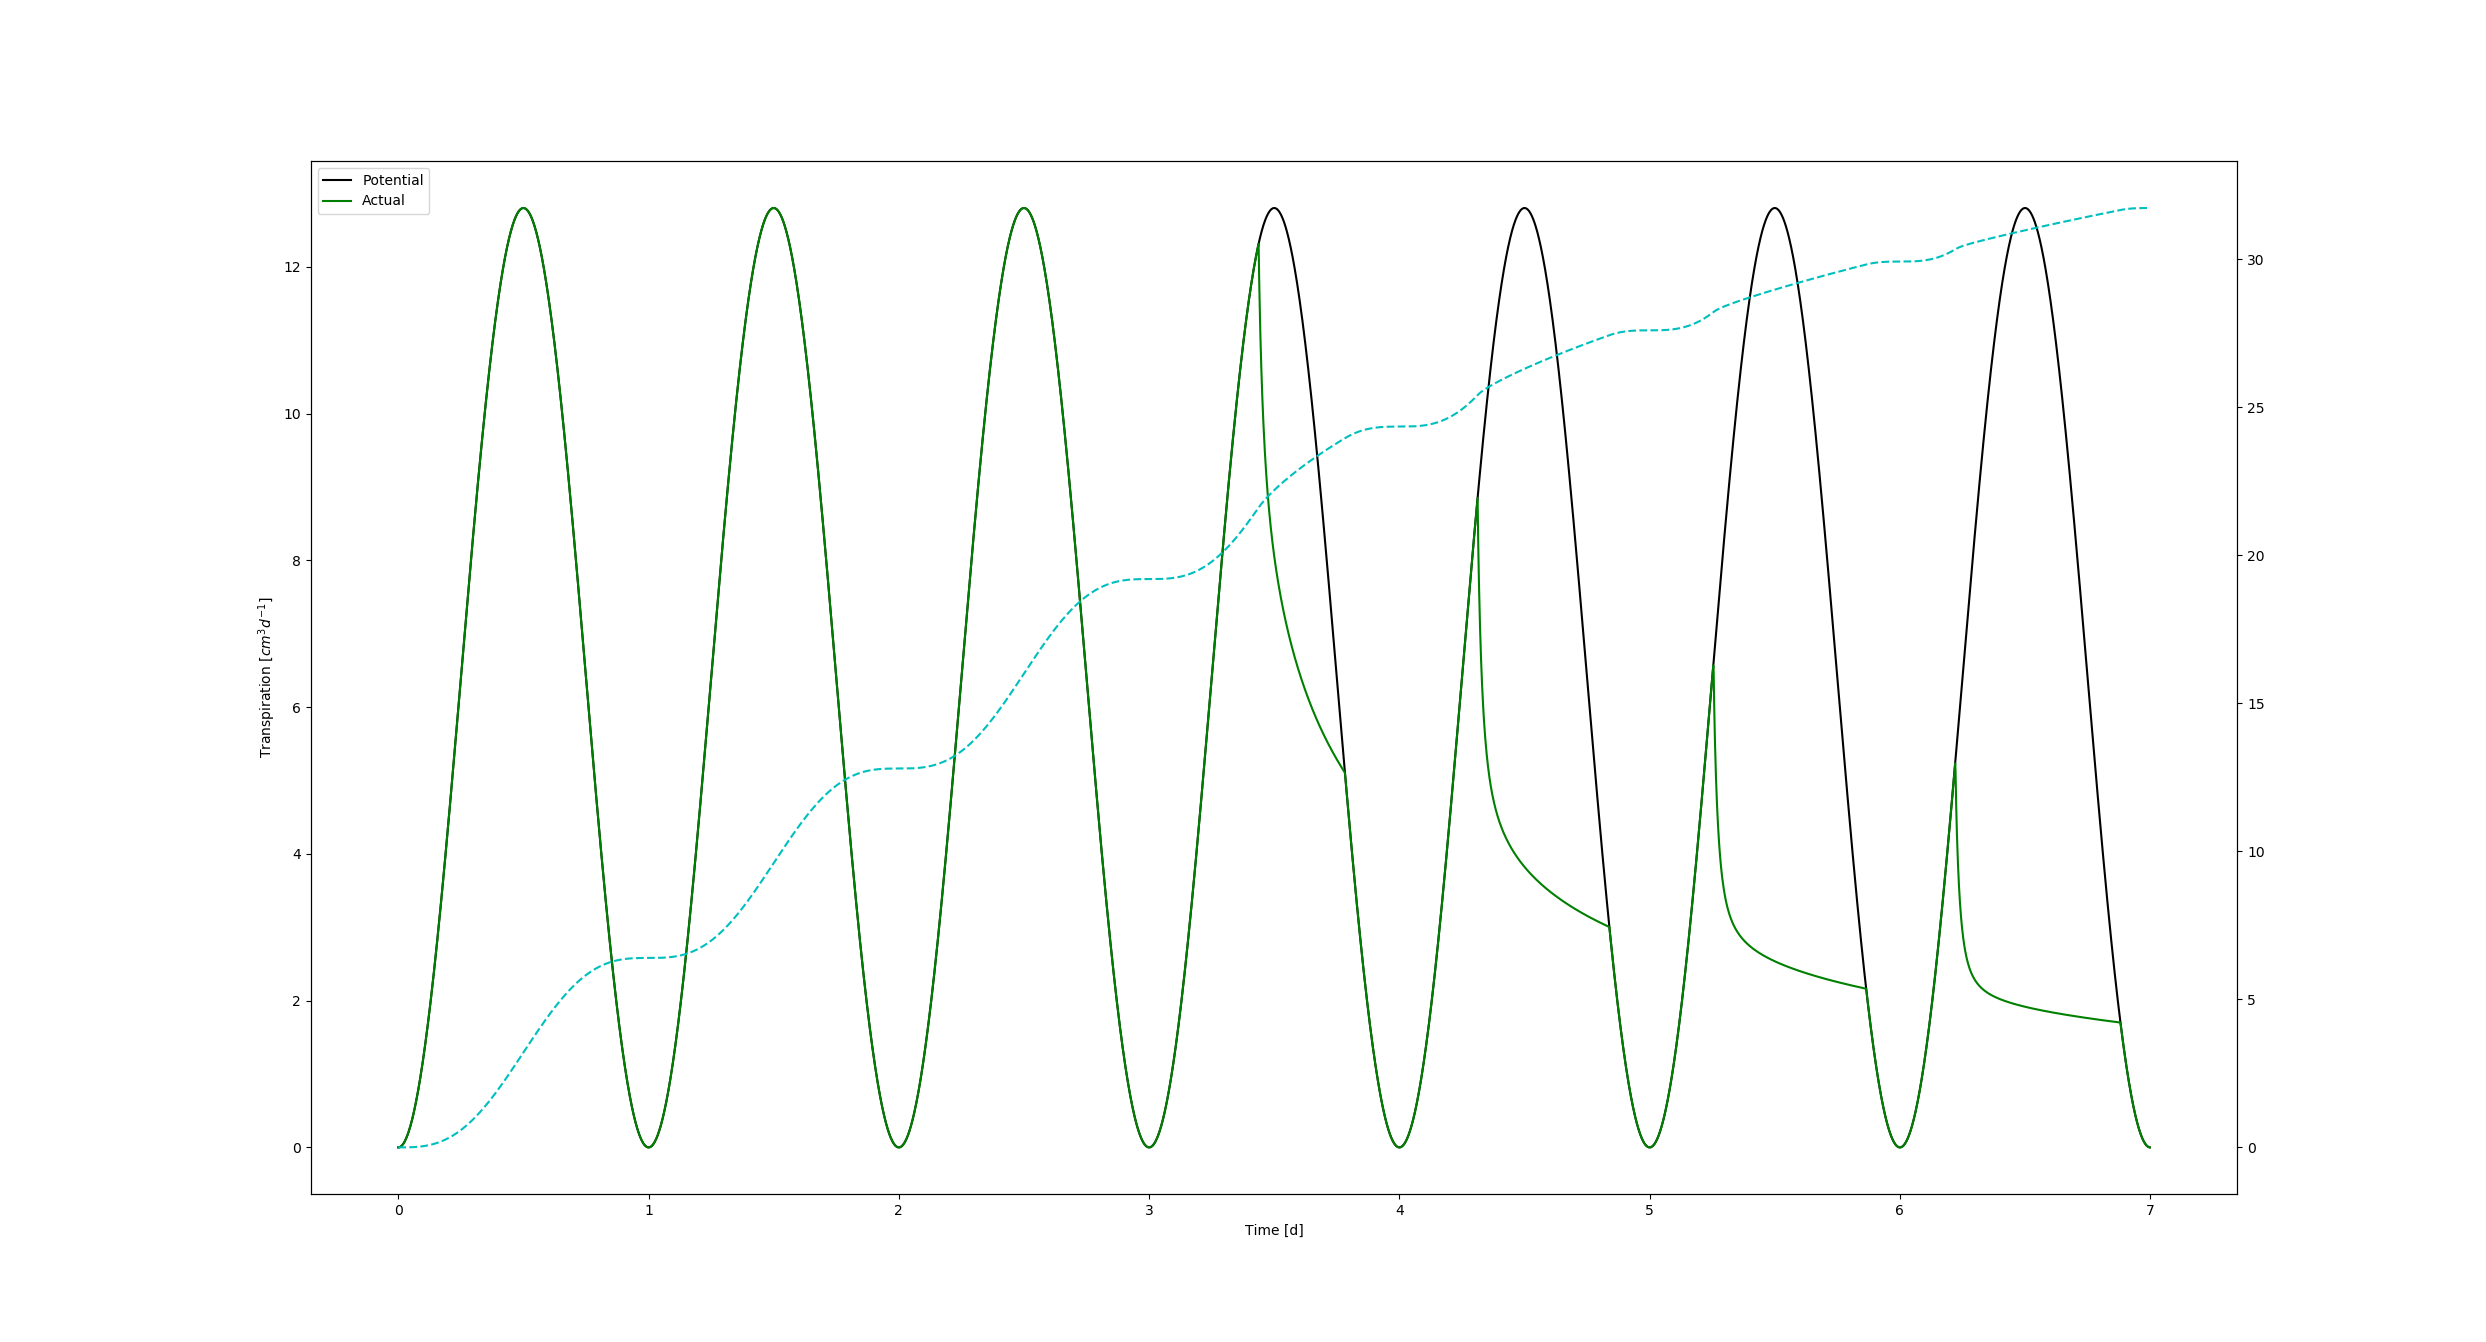
\includegraphics[width=0.99\textwidth]{Figure6c.png}
\subcaption{Confined} \label{fig:uptake_confined}
\end{subfigure}
\begin{subfigure}[c]{1\textwidth}
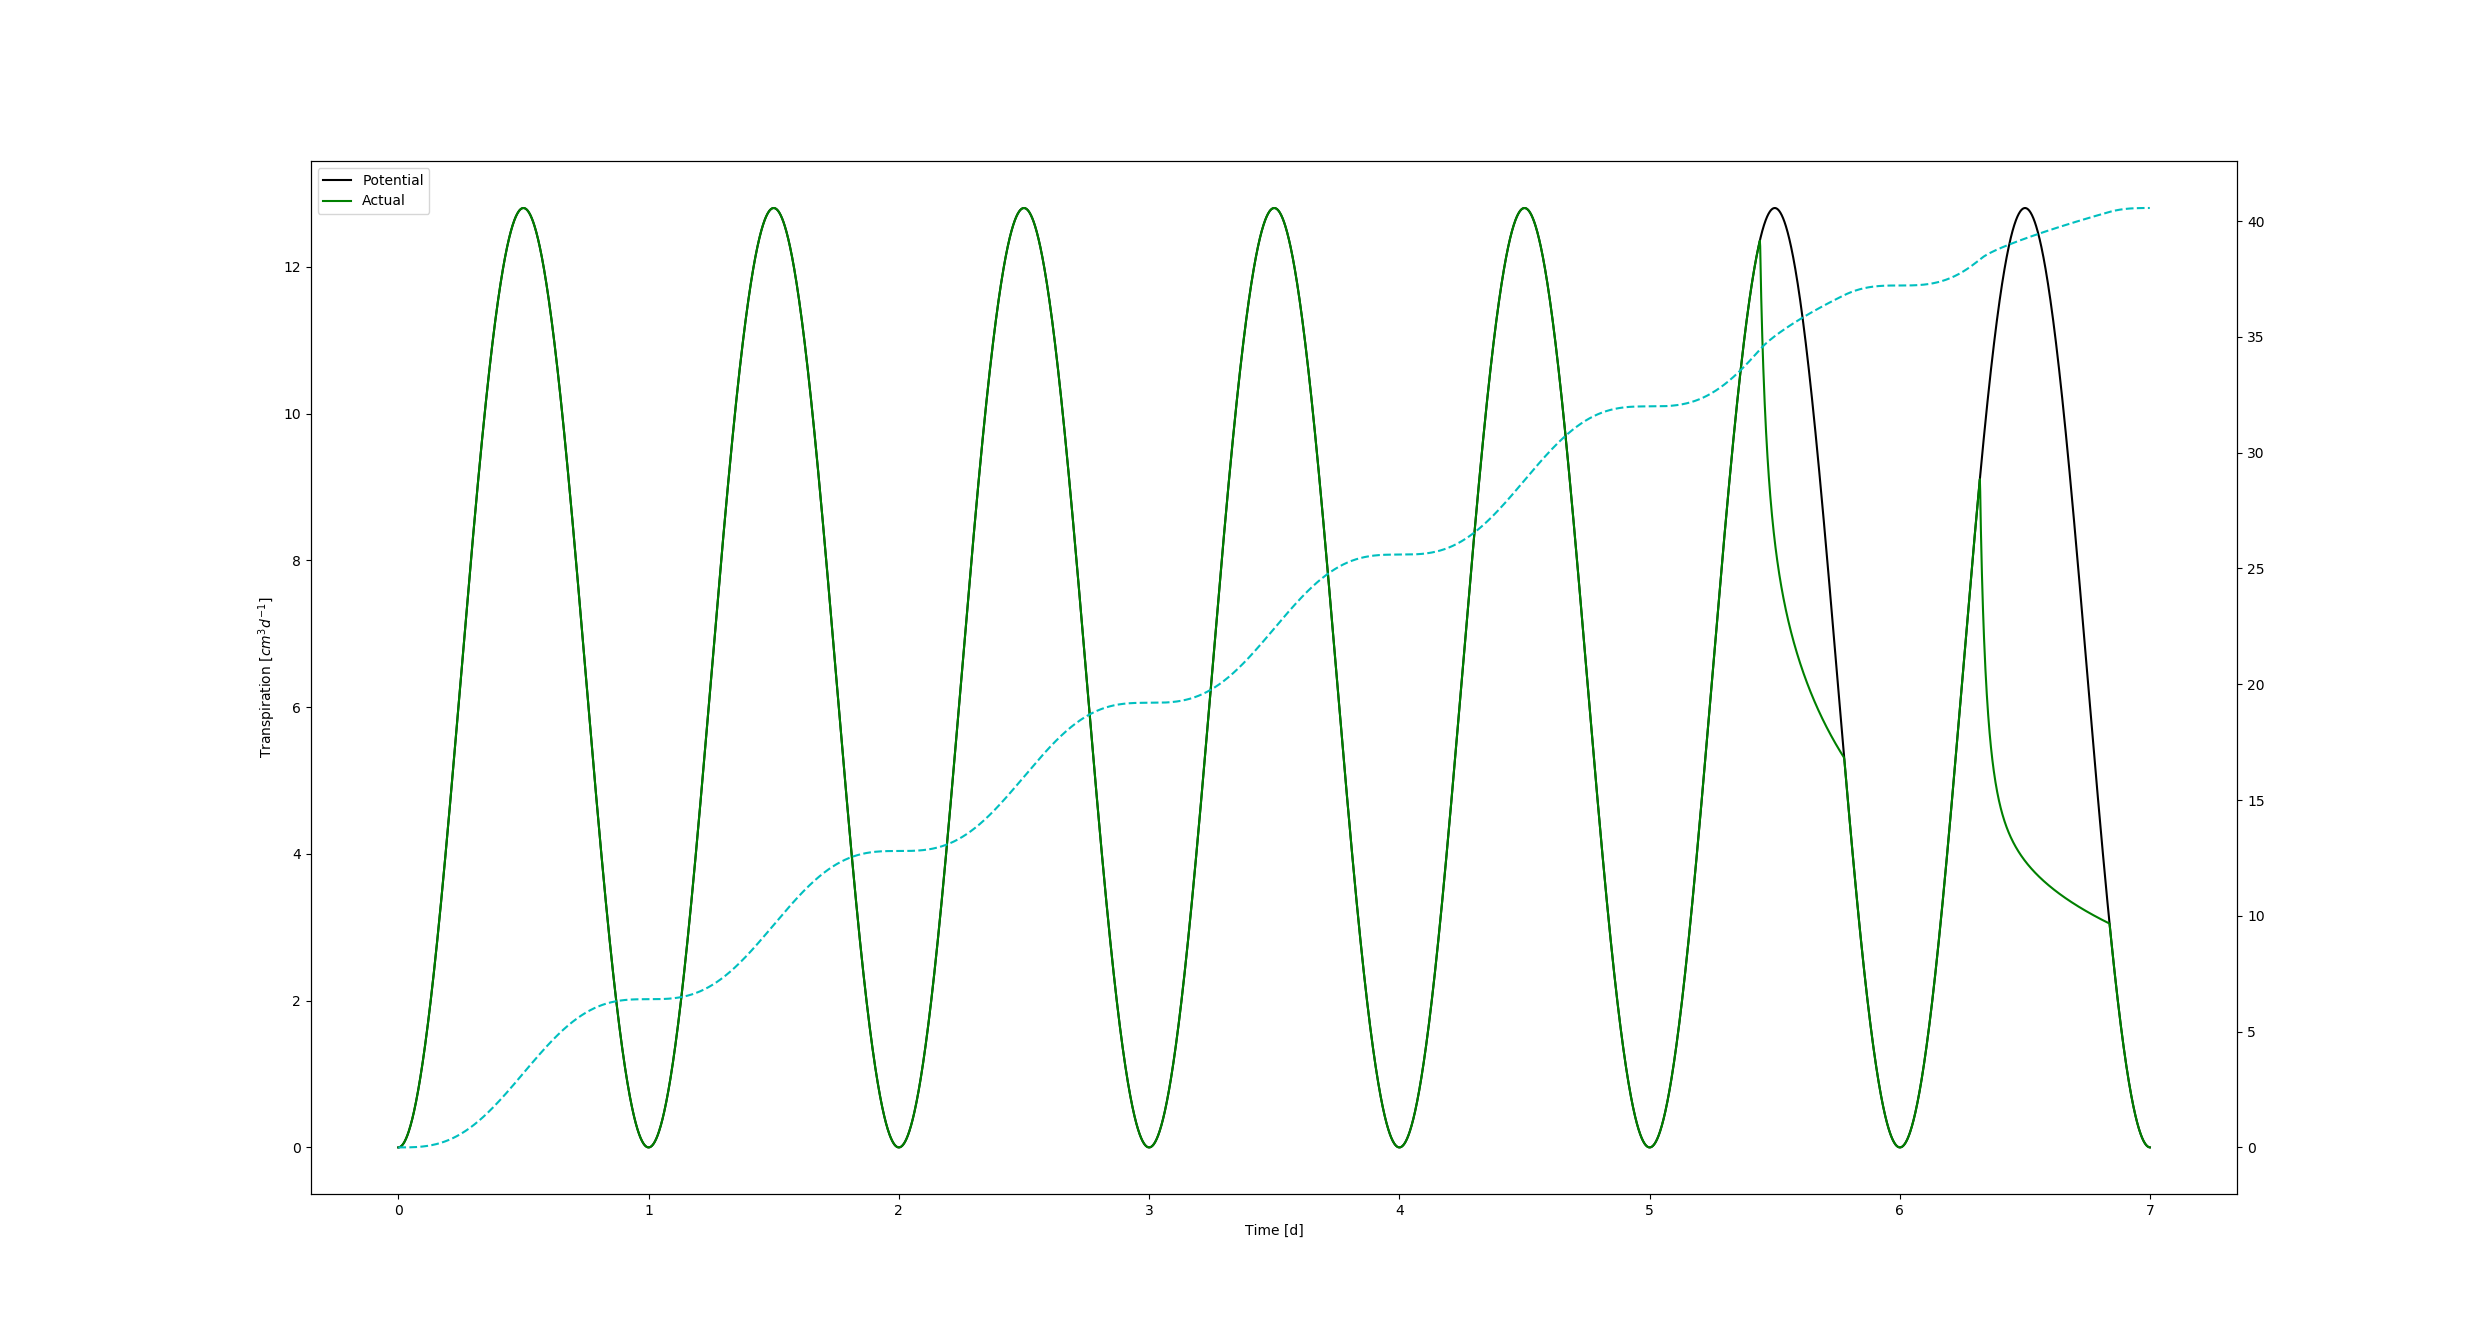
\includegraphics[width=0.99\textwidth]{Figure6c_periodic.png}
\subcaption{Periodic boundary condtions} \label{fig:uptake_peridodic}
\end{subfigure}
\caption{Water uptake and cumulated uptake} \label{fig:uptake}
\end{figure}



